%! TEX root = thesis.tex

\chapter{Theoretical Foundations}%
\label{sec:fundamentals}

Fundamentals / environment and related work: 1/3

\section{Acoustic Modelling}%
\label{sec:acousticmodelling}

\subsection{Spectrograms}%
\label{sec:spectrograms}

Spectrograms are visual representations of frequencies of an audio signal across time scale. In the spectrogram representation, the horizontal axis represents time and the vertical axis the frequencies. The color represents the amplitude of the observed frequencies at a particular point of time. To illustrate, the following image in Figure \ref{fig:spectrogram} shows a spectrogram that has been created from an audio file  \cite{mcfee2015librosa}  . The presence of bright colors at certain places show the amplitude of the frequency at those times in the audio wave. 

\begin{figure}
     \centering
     \begin{subfigure}[b]{0.48\textwidth}
         \centering
         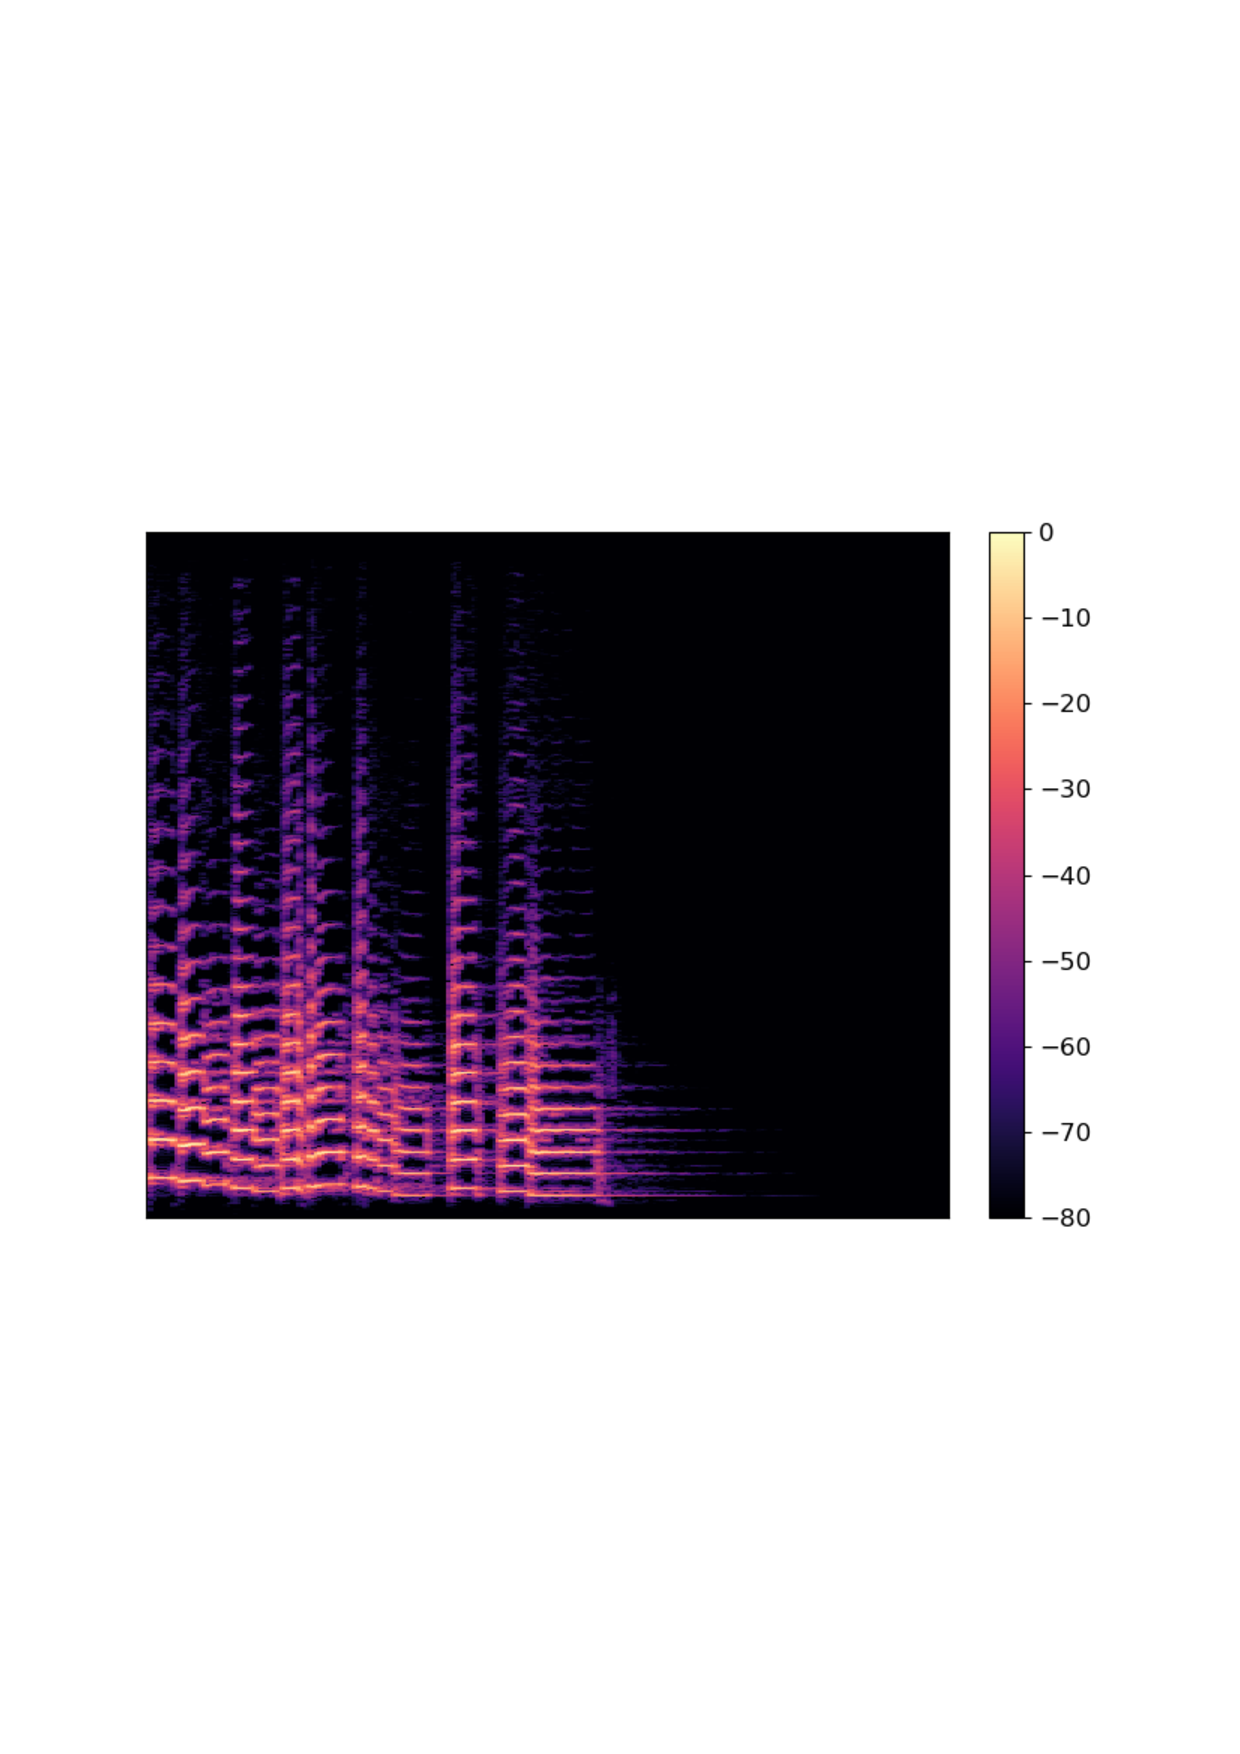
\includegraphics[width=\textwidth]{02-fundamentals/figures/spectrogram.pdf}
         \caption{Spectrogram}
         \label{fig:spectrogram}
     \end{subfigure}
     \hfill
     \begin{subfigure}[b]{0.48\textwidth}
         \centering
         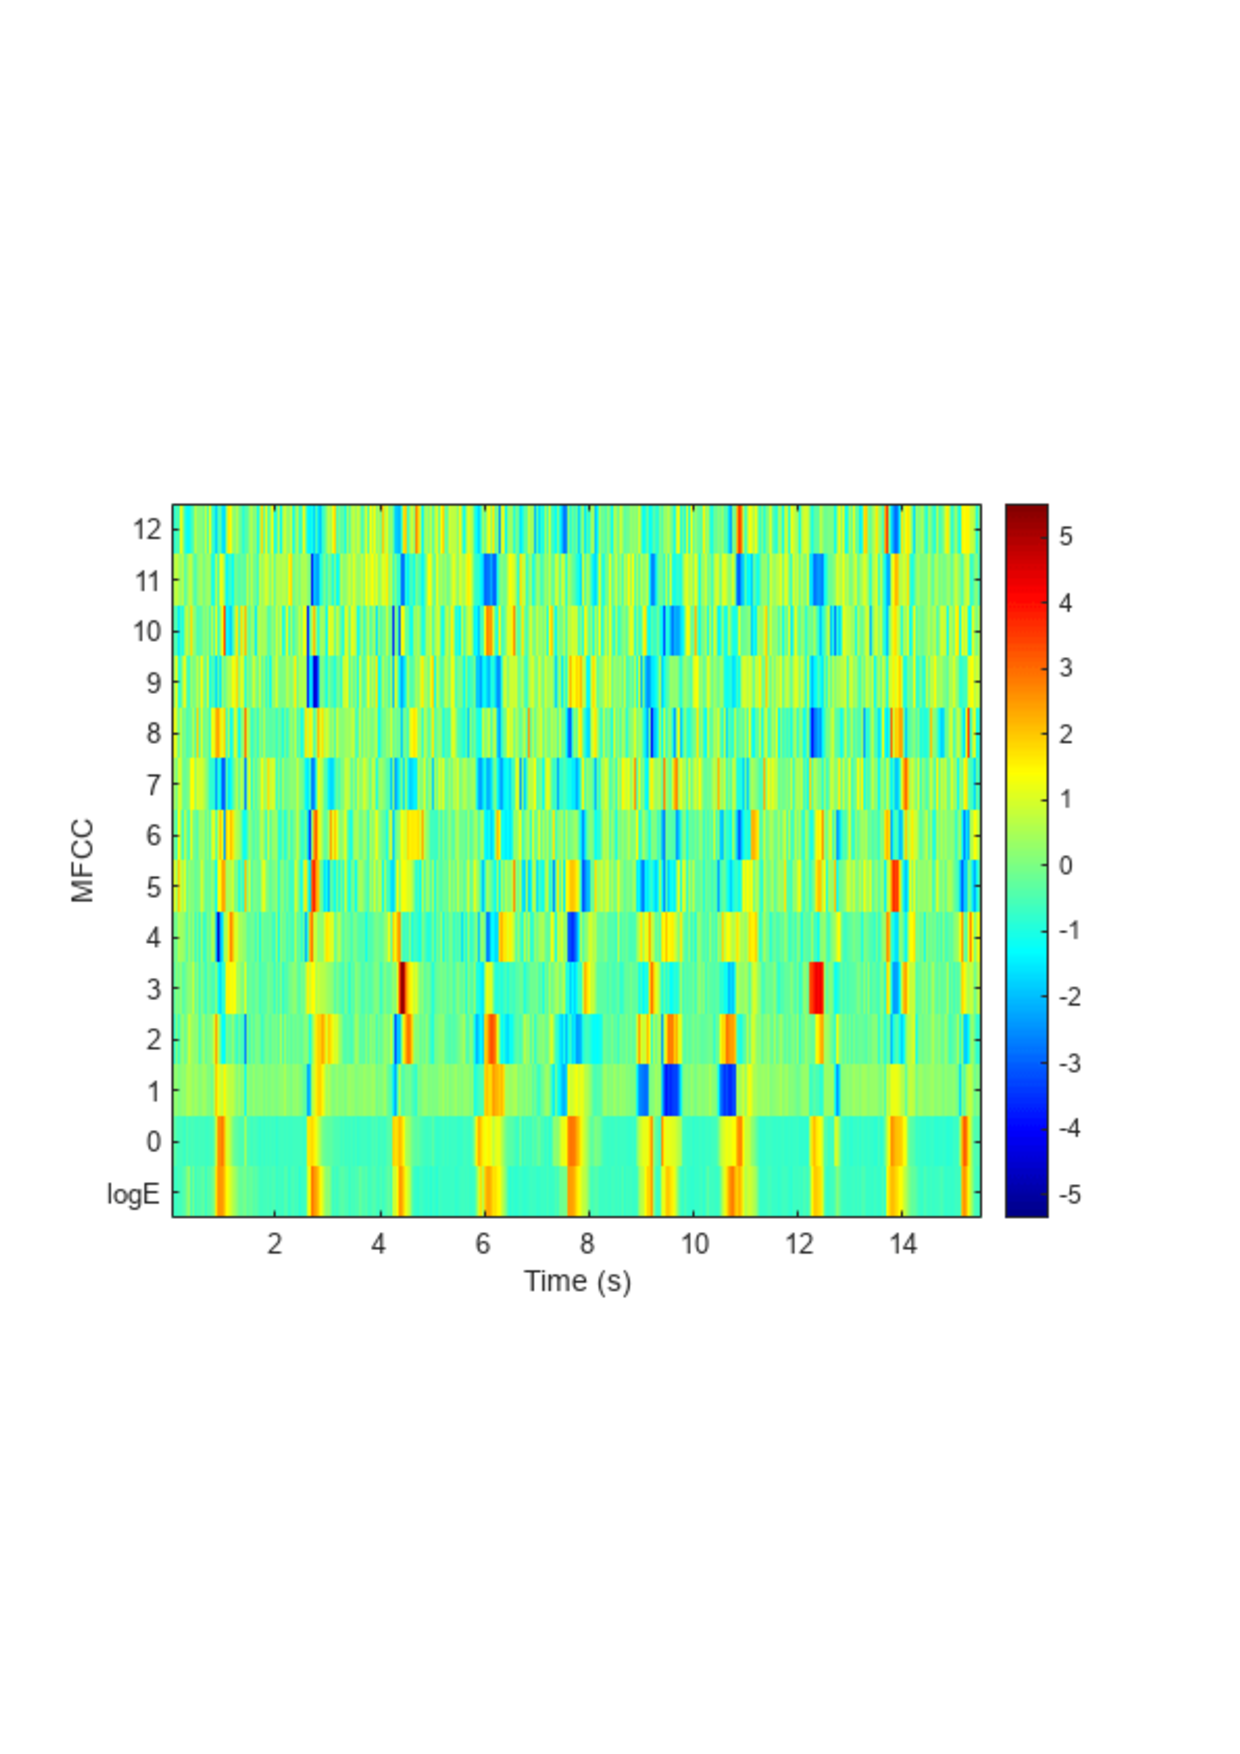
\includegraphics[width=\textwidth]{02-fundamentals/figures/mfcc_matlab.pdf}
         \caption{Mel Frequency Cepstral Coefficients}
         \label{fig:mfcc}
     \end{subfigure}
     \hfill
        \caption{Acoustic Feature Extraction Techniques}
        \label{fig:acoustic_feature_extract}
\end{figure}

In order to create the spectrogram, the audio signal is broken down into smaller frames or windows. Following this, Discrete Fourier Transform (or Fast Fourier Transform) is used on each window to get the frequencies for each window within the time frame of that audio wave. It is also a typical practice to keep overlapping windows so that we don't lose the frequencies. In the Speech recognition or songs lyrics transcription domain, we will be interested in taking windows of 20ms to 30ms as it is roughly the minimum time for a phoneme to be spoken by anyone. This way, we will be able to capture all the phonemes being sung by the singer. Also, typical overlap between two frames is kept at 50\% (typically it is between 25\% and 75\%). Once the fouriers of the windows have been calculated, the absolute values of the complex valued amplitudes are calculated and normalized. The resultant matrix can be plotted and the spectrogram is obtained. 

In ASR systems or Songs Lyrics Transcription, we can convert an audio file into spectrograms in a lossless fashion. When doing so, we can make the problem into an Multiclass Image Classification problem and perform audio transcription. In modern methods such as Whisper, which we will look into later in this chapter, we will see how variants of Spectrograms will be fed into deep learning models to automatically learn a function of the spectrogram to the transcription, allowing for a general approximation of the problem. 

\subsection{Mel Frequency Cepstral Coefficients (MFCC)}%
\label{sec:mfcc}

Cepstral Coefficients (MFCC) are utilized to recuperate sound from a wav sound doc-
ument utilizing different jump lengths and HTK-style Mel frequencies outline of the
above-made sense of steps is plotted in figure 1 underneath. As a general rule, a human
being can hear the sound of 20Hz to 20kHz frequency. A tune of 300 Hz will be as similar
as the sound of a standard dialer tone of a landline telephone. Essentially, a 400 Hz will
sound a piece higher. On contrasting the distance between these two howsoever this
might be seen by your mind will be treated as the practically same [11]. Presently again
the apparent distance of a 900 Hz signal and a 1kHz sound appears to be more prominent
than the initial two albeit the real distinction is something very similar (100Hz). The
Mel scale attempts to catch such contrasts. The fundamental recipe to change over the
recurrence estimated in Hertz (f) into the Mel scale is given by 

\begin{equation}
{Mel}(f)=2595 \log \left(1+\frac{f}{700}\right)
\end{equation}

MFCC coefficients contain information about the rate of change in different spectral bands.


As seen in the Figure \ref{fig:mfccgeneration}, the steps to generate the MFCC are outlined below \cite{huang2001spoken}: 
\begin{itemize}
    \item Frame the signal into short frames.
    \item For each frame calculate the periodogram estimate of the power spectrum.
    \item Apply the mel filterbank to the power spectra, sum the energy in each filter.
    \item Take the logarithm of all filterbank energies.
    \item Take the DCT of the log filterbank energies.
    \item Keep DCT coefficients 2-13, discard the rest.
\end{itemize}

There are a few more things commonly done, sometimes the frame energy is appended to each feature vector. Delta and Delta-Delta features are usually also appended. Liftering is also commonly applied to the final features.

The MFCC model takes the first 12 coefficients of the signal after applying the idft operations. Along with the 12 coefficients, it will take the energy of the signal sample as the feature. It will help in identifying the phones. The formula for the energy of the sample is given below.

Dynamic Features:
Along with these 13 features, the MFCC technique will consider the first order derivative and second order derivatives of the features which constitute another 26 features.

Derivatives are calculated by taking the difference of these coefficients between the samples of the audio signal and it will help in understanding how the transition is occurring.

So overall MFCC technique will generate 39 features from each audio signal sample which are used as input for the speech recognition model.



\begin{figure}
    \centering
    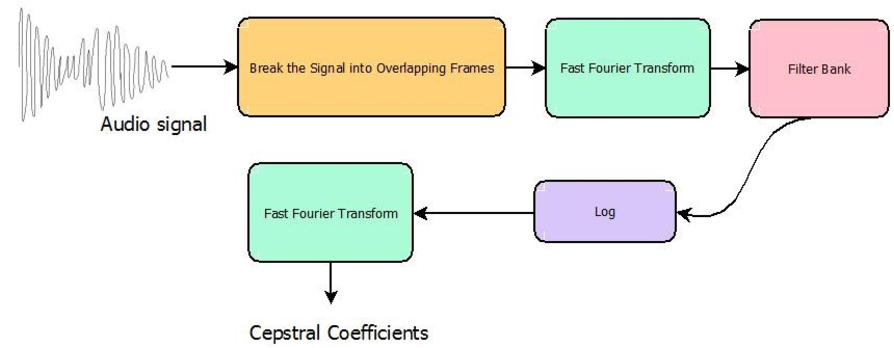
\includegraphics[width=0.9\textwidth]{02-fundamentals/figures/mfcc_generation.pdf}
    \caption{Process to generate MFCC}
    \label{fig:mfccgeneration}
\end{figure}

By the shape of a vocal track, the sound is generated by
a human being. If the shape of the vocal tract can be
resolved precisely then the addressing of the voice tunes
or pitches will be more accurate. Embedding the time
power range of the speech signal and MFCC can detect
the voice. The detailed flowchart is displayed in figure \ref{fig:mfccgeneration}.

An audio signal is constantly changing, so to simplify things we assume that on short time scales the audio signal doesn't change much (when we say it doesn't change, we mean statistically i.e. statistically stationary, obviously the samples are constantly changing on even short time scales). This is why we frame the signal into 20-40ms frames. If the frame is much shorter we don't have enough samples to get a reliable spectral estimate, if it is longer the signal changes too much throughout the frame.

The next step is to calculate the power spectrum of each frame. This is motivated by the human cochlea (an organ in the ear) which vibrates at different spots depending on the frequency of the incoming sounds. Depending on the location in the cochlea that vibrates (which wobbles small hairs), different nerves fire informing the brain that certain frequencies are present. Our periodogram estimate performs a similar job for us, identifying which frequencies are present in the frame.

The periodogram spectral estimate still contains a lot of information not required for Automatic Speech Recognition (ASR). In particular the cochlea can not discern the difference between two closely spaced frequencies. This effect becomes more pronounced as the frequencies increase. For this reason we take clumps of periodogram bins and sum them up to get an idea of how much energy exists in various frequency regions. This is performed by our Mel filterbank: the first filter is very narrow and gives an indication of how much energy exists near 0 Hertz. As the frequencies get higher our filters get wider as we become less concerned about variations. We are only interested in roughly how much energy occurs at each spot. The Mel scale tells us exactly how to space our filterbanks and how wide to make them. See below for how to calculate the spacing.

Once we have the filterbank energies, we take the logarithm of them. This is also motivated by human hearing: we don't hear loudness on a linear scale. Generally to double the percieved volume of a sound we need to put 8 times as much energy into it. This means that large variations in energy may not sound all that different if the sound is loud to begin with. This compression operation makes our features match more closely what humans actually hear. Why the logarithm and not a cube root? The logarithm allows us to use cepstral mean subtraction, which is a channel normalisation technique.

The final step is to compute the DCT of the log filterbank energies. There are 2 main reasons this is performed. Because our filterbanks are all overlapping, the filterbank energies are quite correlated with each other. The DCT decorrelates the energies which means diagonal covariance matrices can be used to model the features in e.g. a HMM classifier. But notice that only 12 of the 26 DCT coefficients are kept. This is because the higher DCT coefficients represent fast changes in the filterbank energies and it turns out that these fast changes actually degrade ASR performance, so we get a small improvement by dropping them.


\subsection{Hidden Markov Models(HMM)}%
\label{sec:hmm}



\section{Automatic Speech Recognition(ASR)}%
\label{sec:automaticspeechrecognition}

Automatic Speech Recognition is a field that started with the Hidden Markov Models (HMM) that are trained using Gaussian Mixture Models (GMM). With the advent of Deep Learning models, new architectures have replaced the existing legacy ones to help calculate better ways to train and convert acoustic elements such as speech into text. In this particular section, we will see the traditional ASR systems and how they work. We will iteratively look at how we can replace existing systems with modern deep learning based modules to improve the effectiveness of the solution.

\subsection{E2E ASR Systems}%
\label{sec:e2easrsystems}

\begin{figure}
    \centering
    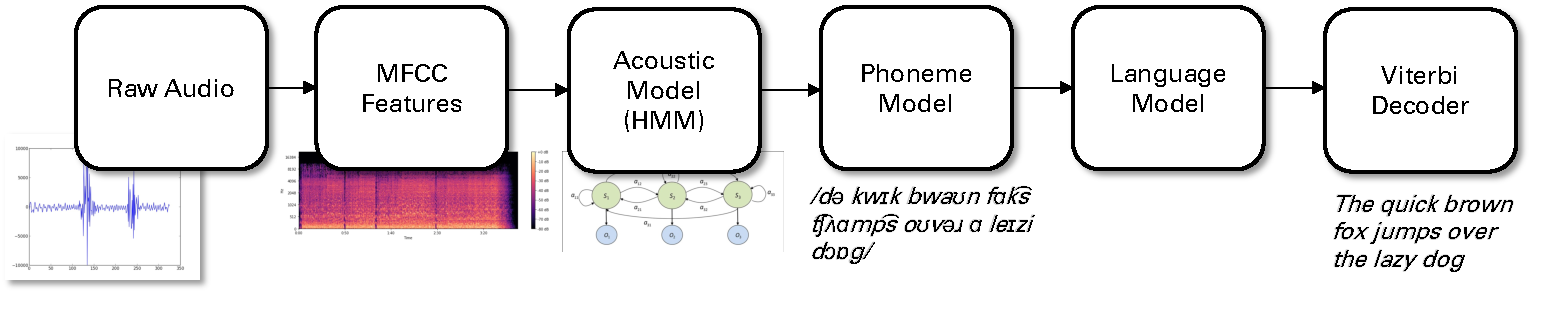
\includegraphics[width=0.9\textwidth]{02-fundamentals/figures/e2e_asr.pdf}
    \caption{End to End Automatic Speech Recognition Systems}
    \label{fig:e2easr}
\end{figure}

\subsection{Wav2Vec2.0 - Self Supervised Approach for Speech Recognition}%
\label{sec:wav2vec2}

\subsection{Whisper - Weak Supervised Learning for Speech Recognition}%
\label{sec:whisper}

\section{Music Information Retrieval (MIR)}%
\label{sec:musicinformationretrieval}

\subsection{Singing Voice Separation (SVS) using DEMUCS}%
\label{sec:demucs}

\section{Decoding Procedures}%
\label{sec:musicinformationretrieval}

\subsection{Language Models (LM)}%
\label{sec:languagemodels}


\subsection{Connectionist Temporal Classification (CTC) Decoder}%
\label{sec:ctcdecoder}


\subsection{Greedy Decoder}%
\label{sec:greedydecoder}

\subsection{Beam Search Decoder}%
\label{sec:beamsearchdecoder}

\section{Hardware Stack}%
\label{sec:hpc}

\section{Software Stack}%
\label{sec:softwarestack}

\section{Discussion}%
\label{sec:foundationaltheorydiscussion}

\begin{itemize}
    \item comment on employed hardware and software
    \item describe methods and techniques that build the basis of your work
    \item review related work(!)

    
\end{itemize}
